\section{Supplement to Section 5: certificates}\label{supp:cert}

This section gives the details of the certificates of Section~\ref{M-sec:certificates} that are not needed to follow the argument: the vertex conditions and the enclosure of the periodic certificate C3, the validation protocols, the effect of the validity bound, what C3 gains over the averaged certificate C2 and how it converges in the number of segments, the results at low radial immersion and the straight-tooth counterexample to averaging.

\subsection{Circle criterion}\label{supp:circle}

The condition of Proposition~\ref{M-prop:circle} was evaluated on a frequency grid of \SI{0.01}{\hertz} over 0.1--\SI{60}{\hertz}, \SI{0.002}{\hertz} over 60--\SI{600}{\hertz} and \SI{0.5}{\hertz} over 600--\SI{5000}{\hertz}, above which $\lvert L\rvert<0.02$. Near $\alim(0)$ the dip of $\operatorname{Re}[1+L(i\omega)]$ is as narrow as the decay rate of the critical root, so the minimum was refined around the eight lowest local minima of $\operatorname{Re}[1+L]$ and the eight highest local maxima of $\lvert L\rvert$ on the grid by three nested zooms of 2001 points each; at 12 test points (four speeds, three depths up to $0.99\alim(0)$) the refinement changed $\mu$ by less than $10^{-5}$ (by at most $2\times10^{-7}$ except at one failing point, $7\times10^{-6}$). The depth $a_{\mathrm{circ}}$ was found by a scan of 39 depths spaced $\alim(0)/40$ followed by bisection to a relative $10^{-6}$. At no speed did a depth pass after a failing one, consistent with the set of depths at which the condition holds being an interval, which at two speeds extends to $\alim(0)$ itself. The condition fails at 124--\SI{196}{\hertz} (median \SI{132}{\hertz}), near the chatter frequency of the uncontrolled cut, whose critical root approaches the imaginary axis; where $a_{\mathrm{circ}}$ is smallest it fails at 124--\SI{129}{\hertz}, near the structural mode. The forced orbit was checked on 2000 depths up to $a_{\mathrm{circ}}$; where the scheduled gain brings the steady command to the clip, Eq.~\eqref{M-eq:feas} holding with equality, a check on 400 depths finds it above \SI{9}{\volt} by at most \SI{5}{\milli\volt}, and the first depth at which it exceeds \SI{9}{\volt} on the 2000-depth grid bounds $a_{\mathrm{circ}}$. With $g=\SI{1500}{\volt\second\per\metre}$ at every speed instead of the scheduled gains, the condition alone holds up to a median over the speeds of $0.954\,\alim(0)$, but the forced orbit is clipped below that depth at 57 speeds (1530--\SI{2090}{\rpm}), down to $0.07\,\alim(0)$ at \SI{1950}{\rpm}.

At the four speeds of Section~\ref{M-sec:bistab-basin}, the depth up to which the frequency condition holds falls slowly with the gain, from 0.986 at $g=\SI{250}{\volt\second\per\metre}$ to $0.862\,\alim(0)$ at $g=\SI{3000}{\volt\second\per\metre}$ at \SI{1420}{\rpm}, and by at most \SI{2}{\percent} over the same range at 1090, 2500 and \SI{2870}{\rpm}. At \SI{1420}{\rpm} the forced orbit itself reaches the clip below that depth for $g\ge\SI{2000}{\volt\second\per\metre}$, so that $a_{\mathrm{circ}}$ is 0.89 and $0.40\,\alim(0)$ at $g=2000$ and 3000; at the other three speeds the orbit stays unclipped. The lower edge of the unsafe band lies above $a_{\mathrm{circ}}$ at all 109 speeds where it was found, by a factor of at least 1.11. The criterion admits any time variation of the sector gain $\varphi(t,y)/y$ in $[0,1]$, whereas in the clipped loop it varies only through $b(t)$ and the deviation itself; this is the source of its conservatism where it fails well below $\alim(0)$. The Popov criterion, which would use more of the structure, requires a time-invariant nonlinearity and does not apply while $b(t)\neq0$.
% src: verification/paper/circle_criterion.py (F_HZ grid, mu, _zoom, a_circ, first_clipped_depth, add_orbit_limit), circle_criterion.json (g_best: orbit_peak_V_up_to_a_circ - 9 V <= 0.0046 V; g1500: ratio_median 0.9537, n_orbit_limited 57, rpm 1530-2090, ratio_eff_min 0.0724 at 1950 rpm; refinement_check: |mu_grid - mu_refined| <= 1.8e-7 at 11 points, 7.2e-6 at 1090 rpm 1.25 mm (failing); g_best: n_nonmonotone 0, n_reached_a0 2; verification/paper/circle_gainsweep_orbit.py/.json (f_fail: 123.7-195.5 Hz, median 131.7; gain_sweep ratio_eff at 1420 rpm 0.889 (g 2000), 0.402 (g 3000), unchanged elsewhere); gain_sweep: 1420 rpm 0.9856 at g = 250 to 0.8617 at g = 3000; 1090 rpm 0.9978-0.9780, 2500 rpm 0.9991-0.9898, 2870 rpm 0.99996-0.99951; band: edge_over_a_circ_min 1.1085, all_edges_above_a_circ true)

\paragraph{Proof on the continuous frequency axis} The proof was made at the scheduled gains of Section~\ref{M-sec:feasibility} (the results for $g=\SI{1500}{\volt\second\per\metre}$ and the gain sweep above rest on the grid). Let $a_\mu$ be the depth found by the bisection above, up to which the frequency condition holds; $a_\mu=a_{\mathrm{circ}}$ except at the 44 speeds where the forced orbit reaches the clip first, where $a_\mu$ is 1.14--4.6 times $a_{\mathrm{circ}}$. With $s=i\omega$, $L=h/B$ with $h=-igK_a\omega^3/A$, $A=\omega_a^2-\omega^2+i\,2\zeta_a\omega_a\omega$ and $B=k-m\omega^2+ic\omega-\overline{aH}\,(1-\cos\omega T+i\sin\omega T)$, so that $\operatorname{Re}[1+L]=\mathcal N/\lvert B\rvert^2$ with $\mathcal N=\lvert B+h/2\rvert^2-\lvert h\rvert^2/4$; $\mathcal N>0$ on a box proves $\operatorname{Re}[1+L]>0$ there and $B\neq0$. This quantity was enclosed on boxes $[\omega_1,\omega_2]\times[a_1,a_2]$ by interval arithmetic in double precision: every addition, multiplication and division rounded outwards by one unit in the last place, cosine and sine bounded by their values at the ends of the interval, padded by $2^{-50}$, and by $\pm1$ wherever an extremum may lie inside, and the model constants taken as intervals of relative half-width $10^{-12}$; a self-test at start-up checks the enclosures against the floating-point $L$ and the cosine and sine used against the C library. Starting from frequency intervals of at most \SI{0.25}{\radian} of $\omega T$ over $[0,2\pi\cdot5000]$\,rad/s, each with the whole depth range $[0,(1-10^{-3})\,a_\mu]$, boxes with a non-positive lower bound were bisected, in frequency or in depth, until every box had a positive lower bound (785--5500 box evaluations per speed; no undecided box at any of the 251 speeds); boxes whose bound was below 0.99 times the grid value of $\mu$, or of $\operatorname{Re}[1+L]$ at the box centre, were then bisected further, for 1200--30\,000 evaluations per speed in all. For $\omega\ge2\pi\cdot\SI{5000}{\radian\per\second}$, $\lvert A\rvert\ge\omega^2-\omega_a^2$ and $\lvert B\rvert\ge m\omega^2-k-2\lvert\overline{aH}\rvert$ give a bound on $\lvert L\rvert$ that decreases with $\omega$ and is at most 0.0071. After the tightening, the smallest certified lower bound of $\operatorname{Re}[1+L]$ over a speed's boxes is 0.00098 at the hardest speed (\SI{950}{\rpm}) and 0.043 at the median one. Because $B\neq0$ on the whole axis for every depth up to $(1-10^{-3})\,a_\mu$ and the cut is stable at $a=0$, the proof also shows that these depths lie below $\alim(0)$. At the smaller of $(1+10^{-3})\,a_\mu$ and the midpoint between $a_\mu$ and $\alim(0)$, the enclosure at the grid minimiser has a negative upper bound at 249 speeds, so the depth at which the frequency condition stops holding is located to within $10^{-3}$; at 2990 and \SI{3000}{\rpm} the condition holds up to $\alim(0)$. The proof covers the averaged model with the constants of the code and relies on the documented error of the C library's cosine and sine; the second hypothesis of Proposition~\ref{M-prop:circle}, an unclipped forced orbit, rests on the closed-form command on 2000 depths, and at the 44 speeds where it fails first it sets $a_{\mathrm{circ}}$.
% src: verification/paper/circle_interval.py (docstring: algebra, intervals, phases, tail, fail check), circle_interval.json, circle_interval.log (251 verified, undecided 0; boxes 1210-29721 per speed; min_lb min 9.8e-4, median 0.0434; tail 7.06e-3; fail check confirmed 249, n/a 2 at 2990 and 3000 rpm); rows: n_box_evals_phase1 785-5454, n_box_evals 1210-29721, min_lb_phase1 min 2.8e-7, min_lb (after tightening) min 9.8e-4 at 950 rpm; a_v_mm = 0.999 a_circ_mm (condition-only depth, circle_criterion.json g_best a_circ_mm), which exceeds a_circ_eff_mm at the 44 orbit-limited speeds 1530-1990 rpm by 1.14-4.57 times; fail point a_f = min(1.001 a_circ_mm, (a_circ_mm + a0)/2); circle_criterion.py: max_orbit_peak_V_up_to_a_circ 9.00463 V from orbit_peak_V_up_to (400 depths), first_clipped_depth on 2000 depths

\subsection{Loss of contact as a second sector condition}\label{supp:contact}

On the engaged arc of half-immersion down milling, $\phi\in[\pi/2,\pi]$, the chip of a slice is $h=f_z\sin\phi+r\lvert\cos\phi\rvert$ with $r=\tilde x-\tilde x(t-T)$ [Eq.~\eqref{M-eq:chip}], so loss of contact occurs only for $r<0$, where $f_z\sin\phi<\lvert r\rvert\lvert\cos\phi\rvert$. The force lost by a slice, $(K_{tc}\sin\phi+K_{rc}\lvert\cos\phi\rvert)\max\{\lvert\cos\phi\rvert\lvert r\rvert-f_z\sin\phi,0\}$, has the sign of the linear regenerative force and is convex in $\lvert r\rvert$, so its ratio to $\lvert\overline{aH}\,r\rvert$ grows with $\lvert r\rvert$ and is largest at $\lvert r\rvert=\delta f_z$. Its largest value over the tooth period, with the helix ($2^{18}$ instants, quadrature error of about $1.3\times10^{-4}$), is $\theta(a,\delta)$: 0.14--0.60 over the 48 depths of Section~\ref{M-sec:cert-c2} at $\delta=0.5$ (largest at shallow depths, where few slices are engaged), 0.17--0.23 at the 12 points of Section~\ref{M-sec:cert-lmi}; its average over the arc is 0.139.

With $\theta=0$ the extended conditions reproduce C2: they give 3.0579 against \SI{3.0578}{\milli\metre\per\second} at \SI{2500}{\rpm} and $0.9\alim$, and the blocks agree bit for bit. Perturbed candidates (multiplier $S_2$ scaled by $10^{\pm3}$ or negative, $\theta$ tripled, the sign of the new column reversed) are rejected by the check. Runs of the collocation model from boundary points of a certified ellipsoid, with the true dead zone and the true lost force, stayed inside it (largest $\mathcal V=0.998$). At $0.9\alim$, with the arc-averaged share 0.139 instead of $\theta$, the certified kick would be 0.89--\SI{0.95}{} times that without loss of contact; with $\delta=1$, where $\theta$ is 0.35--0.40, no certificate exists at \SI{1090}{\rpm} and only a vanishing one (\SI{0.005}{\milli\metre\per\second}) at \SI{2500}{\rpm}, so the larger validity bound does not pay once loss of contact is included.
% src: verification/paper/contact_sector.py/.json (theta: n_tgrid 262144, quadrature_check max rel err 1.3e-4, theta_05_range_48 0.140-0.604, theta_bar_05 0.1394; tests.theta0_reproduction 3.0579046/3.0577848 mm/s, blocks bitwise identical; negative tests rejected; sampled run max_V 0.998; campaign.tradeoff_090: beta2 with theta_bar 5.526/3.543/2.870/6.538 against beta1 6.196/3.843/3.058/6.892 mm/s; delta 1: theta 0.399/0.400/0.391/0.347, beta2 0/2.881/0.005/5.969)

\subsection{Proof of the periodic certificate and details of the C2 results}\label{supp:proof-c3}

\paragraph{Proof of Proposition~\ref{prop:c3}} As $\mathcal A(t)W(t)$ contains $s$, $s^2$ and $rs$, the matrix of Eq.~\eqref{eq:lmi-per}, with $\sigma$ for $s^2$, is affine in $(s,\sigma)$ for fixed $r$ and in $r$ for fixed $(s,\sigma)$; since $(s,s^2)$, $s\in[0,1]$, lies in the triangle spanned by the three points, its value at any $t$ of the segment is a convex combination of the six vertex values. Equations~\eqref{M-eq:lmi-incl}--\eqref{M-eq:lmi-size} are affine in $(W,Y)$, so they hold on segment $k$ with the level $u_{0,k}\le\Vmax-\lvert b(t)\rvert$. The proof of Proposition~\ref{M-prop:c2} then applies on each segment, $\Delta_kW$ accounting for the variation of $W$, and $\mathcal V$ is continuous across the nodes.


\paragraph{Step entry and gain map} The step entry is certified only at $0.3\alim$ at 1090, 1420 and \SI{2870}{\rpm} ($\beta=1.04$--1.61), never at \SI{2500}{\rpm}, and always below the simulated step-entry limits (0.75--$0.90\alim$); at 0.5--$0.9\alim$, $\beta=0.16$--0.72, so no productive depth is certified. Over the gain map of Section~\ref{M-sec:feasibility} (42 speeds, seven depths from 0.5 to $0.98\alim$), 287 of 294 points were certified, with certified kicks of 0--\SI{16}{\milli\metre\per\second} (median 6.6) at $0.9\alim$; the other seven lie at 1520--\SI{2000}{\rpm}, where the gain sits at or near the authority limit and the forced orbit itself saturates ($u_0\le0$, three points) or leaves $u_0=0.04$--\SI{0.38}{\volt}, too little for any candidate to pass the check (Fig.~\ref{fig:surf}).
% src: README §12.5, §12.6; results/c2_step.npz, c2_summary.json (step: td_step_limit_frac 0.895/0.893/0.754/0.821), c3_summary.json (errata.c2_step); results/c2_surface.npz (cert, u0, msg), c2_summary.json (surface), c3_summary.json (errata.c2_surface: 0-16.02, median 6.58)

\subsection{Vertex conditions and enclosure of the periodic certificate}\label{supp:cert-vertex}

On segment $k$, with $W(s)$ and $Y(s)$ from Eq.~\eqref{eq:Wt}, the decrease condition~\eqref{eq:lmi-per} is imposed at the six vertices of Proposition~\ref{prop:c3}, $(s,\sigma)=(0,0)$, $(\tfrac12,0)$ or $(1,1)$ and $r=\pm\varepsilon_k$, as
\begin{equation}\label{eq:app-per}
\begin{bmatrix}\Delta_kW-\Lambda-\Lambda^\top-2\lambda W(s) & BS_k-Y(s)^\top\\ S_kB^\top-Y(s) & 2S_k\end{bmatrix}\succ0,
\end{equation}
where $\Lambda=(A_0+Bk^\top)\,W(s)+E_r\,\big[\nu_0W_k+\nu_1W_{k+1}\big]$, $\nu_0=(c_{0,k}+r)(1-s)+c_{1,k}(s-\sigma)$ and $\nu_1=(c_{0,k}+r)s+c_{1,k}\sigma$; these reproduce $aH(t)W(t)$ exactly when $\sigma=s^2$. Since $E_r=p_rq_r^\top$, with $p_r=e_2/m$ and $q_r=e_1-e_{4+N}$, has rank one, the part of the matrix of Eq.~\eqref{eq:app-per} that depends on $r$ is $-r(\bar p\bar v^\top+\bar v\bar p^\top)$, with $\bar p=[p_r^\top\ 0]^\top$ and $\bar v=[(W(s)q_r)^\top\ 0]^\top$. By Petersen's lemma, exact for a scalar uncertainty \citep{petersen1987stabilization}, the matrix is positive definite for all $\lvert r\rvert\le\varepsilon_k$ if and only if, for some $\varkappa>0$,
\begin{equation}\label{eq:app-merged}
\begin{bmatrix}M_0-\varkappa\bar p\bar p^\top & \varepsilon_k\bar v\\ \varepsilon_k\bar v^\top & \varkappa\end{bmatrix}\succ0,
\end{equation}
with $M_0$ the matrix at $r=0$. Condition~\eqref{eq:app-merged} merges the vertices $r=\pm\varepsilon_k$ and leaves three LMIs per segment; for balance, $p_r$ is divided and $q_r$ multiplied by $10\,\big(\lVert p_r\rVert/(\lVert q_r\rVert\varepsilon_k)\big)^{1/2}$. The independent check tests the six vertices separately, with a round-off scale that also includes $\big(\lVert A_0+Bk^\top\rVert+(\lvert\nu_0\rvert+\lvert\nu_1\rvert)\lVert E_r\rVert\big)\max(\lVert W_k\rVert,\lVert W_{k+1}\rVert)$ and $(\lVert W_k\rVert+\lVert W_{k+1}\rVert)/\tau_s$, to cover rounding in $\Delta_kW$ and in $\mathcal AW$.

The line $c_{0,k}+c_{1,k}s$ is fitted by least squares to $aH$ at the midpoints of 2048 equal cells of segment $k$, and $\varepsilon_k$ is the largest residual plus $(\Upsilon+\lvert c_{1,k}\rvert/\tau_s)\,\tau_s/4096$, where $\Upsilon\ge\lvert\mathrm d(aH)/\mathrm dt\rvert$ holds because each tooth contributes to $\mathrm d(aH)/\mathrm dt$ only through the two ends of its engaged interval in $z$.
% src: src/c3_periodic.py (enclosure: N_ENC 2048; aH_rate_bound; corners; lmi: merged block, P_SCALE 10; check); README §14.2, §14.9

\subsection{Certified kick over the gain map}\label{supp:cert-surface}

Figure~\ref{fig:surf} shows the certified kick of the averaged model over the gain map of Section~\ref{M-sec:feasibility} and the step-entry certificate at the four speeds of Section~\ref{M-sec:cert-c2}.

\begin{figure}[!htbp]
\centering
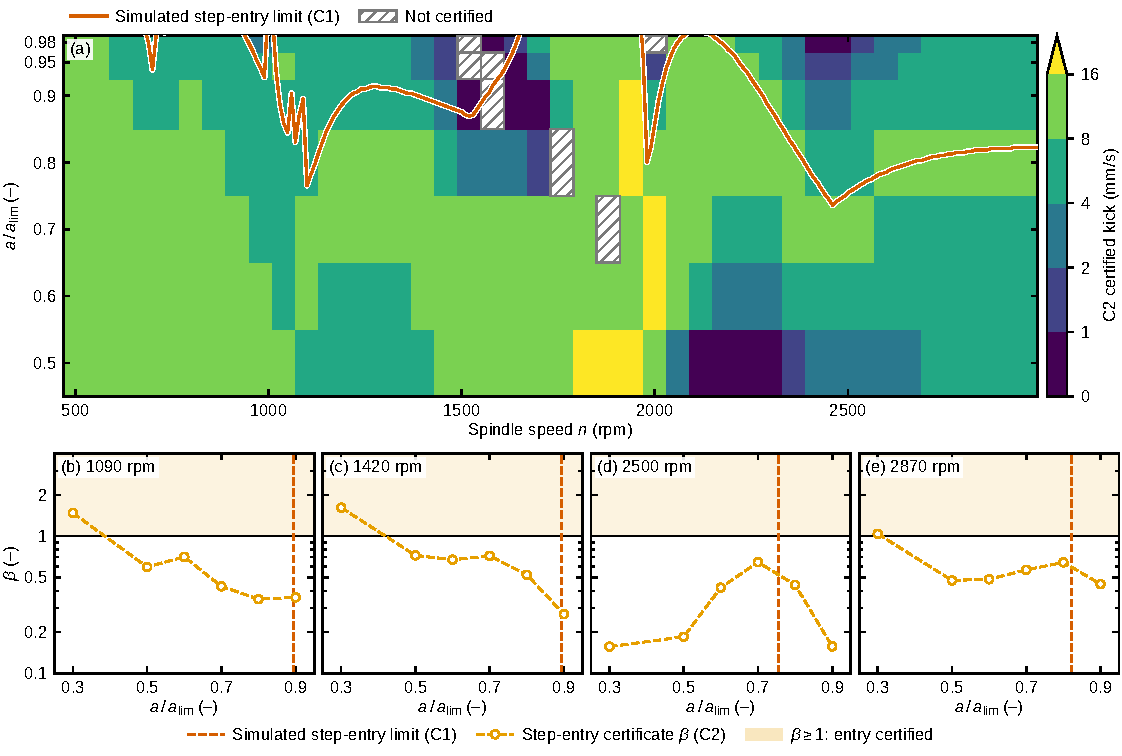
\includegraphics[width=\textwidth]{figures/fig07_certified_surface.pdf}
\caption{(a) Certified kick of the averaged model (C2) over spindle speed and depth on the gain map of Section~\ref{M-sec:feasibility}: 42 speeds and the seven computed depths 0.5, 0.6, 0.7, 0.8, 0.9, 0.95 and $0.98\alim$, drawn as rows of equal height (the vertical axis is not to scale in $a/\alim$), with colour bins in a 1--2--5 sequence. Not certified (7 of 294 points): cross-hatched, the forced orbit itself reaches the clip ($u_0\le0$, three points); hatched, no candidate passed the check (four points). Open circles: depths above the simulated step-entry limit of Section~\ref{M-sec:bistability}, at which the step entry from rest ends in chatter. (b)--(e) Step-entry certificate $\beta$ at the four speeds of Fig.~\ref{M-fig:cert}; $\beta\ge1$ (shaded) certifies the entry at rest on a fresh surface at the entry phase of the simulator; dashed: simulated step-entry limit. Command bound corrected as in Section~\ref{M-sec:cert-lmi}.}
\label{fig:surf}
\end{figure}

\subsection{Validation protocols}\label{supp:cert-protocol}

The off-axis test used boundary points of the certified ellipsoid (for C3, of the ellipsoid at the phase of application) in 18 directions: both signs of the points that maximise $\tilde x$, $\dot{\tilde x}$, $\tilde q$, $\dot{\tilde q}$, $\tilde x(t-T)$ and $\tilde x-\tilde x(t-T)$ on it, and six random points. They were applied in the simulator as full-state deviations at four phases a quarter of a tooth period apart, with the protocol of Section~\ref{app:lmi}. These directions were sampled, not searched for the worst case.

The sampled check followed 48 trajectories per point of the collocated model with the true dead zone over 40 tooth periods, started at 0.999 of the boundary in random directions and phases. $\mathcal V$ never exceeded its initial value 0.998 for C2 and stayed below 0.997 after the first step for C3 (2256 starts). This is only a consistency check, as ellipsoids that are too large can pass it; the certificates rest on the independent check of Section~\ref{M-sec:cert-check}.

Floquet limits of the periodic collocated model used 200 Magnus steps per period and bisection to a relative $10^{-5}$. With $N+8$ nodes the spectral radius at the computed limit differs from 1 by at most $6\times10^{-6}$, and at nine speeds at half immersion the limit agrees with stored semi-discretisation limits \citep{insperger2002semi,insperger2004updated} within $1.3\times10^{-5}$; no such check was made at $a_e/D=0.1$.
% src: src/c2_certificate.py (boundary_directions, deviation_to_pert, td_offaxis, proof_check: nruns 48, nper 40); src/c3_periodic.py (td_offaxis, floquet_a_lim); results/c2_validate.npz (proof_vmax 0.998001, offaxis 0/3456); results/c3_summary.json (basin: proof_starts 2256, proof_vmax 0.9969, offaxis 0/3384); results/c3_floquet.npz (rho_n8: 4.9e-6, 5.5e-6); README §14.4 (SDM agreement 1.3e-5 at nine speeds)

\subsection{Validity bound}\label{supp:cert-delta}

Without the validity bound~\eqref{M-eq:lmi-valid}, the certified ellipsoid at \SI{2500}{\rpm} and $0.7\alim$ admitted histories displaced by 7--12 feeds, with the tool entirely out of the cut. These states return to the orbit in the linear model, but 32 of 72 off-axis runs from its boundary ended in chatter in the simulator, against none with the bound. Table~\ref{tab:delta} gives the certified kick for other values of $\delta$ and without the bound, with the command bound of the original C2 solves. Near the limit the sector condition sets the certificate and $\delta$ hardly matters; at shallow depths the bound sets it, and without the bound $\beta$ doubles at \SI{1090}{\rpm} and $0.15\alim$, but the set may then contain states with the tool out of the cut, as above.
% src: README §12.4 (7-12 f_z; 32 of 72 runs, 0 of 72 with the bound); verification/paper/revision_runs.json (beta_vs_delta; 23.367/11.689 = 2.0 at 1090 rpm, 0.15 a_lim; delta = 0.5 values equal results/c2_validate.npz cert)

\begin{table}[!tbp]
\centering
\caption{Certified kick $\beta$ (\si{\milli\metre\per\second}) of the averaged model (C2) against the validity bound $\delta$ of Eq.~\eqref{M-eq:lmi-valid}; $\delta=0.5$ is used in the article.}
\label{tab:delta}
\small
\begin{tabular}{@{}lcccc@{}}
\toprule
Point & $\delta=0.25$ & $\delta=0.5$ & $\delta=1$ & no bound\\
\midrule
\SI{1090}{\rpm}, $0.15\alim$ & 6.57 & 11.7 & 18.5 & 23.4\\
\SI{2870}{\rpm}, $0.3\alim$ & 5.69 & 8.74 & 10.0 & 10.4\\
\SI{2500}{\rpm}, $0.9\alim$ & 2.90 & 3.06 & 3.07 & 3.07\\
\bottomrule
\end{tabular}
\end{table}
% src: verification/paper/revision_runs.json (beta_vs_delta: 6.5748/11.6891/18.4958/23.3672; 5.6854/8.7429/10.0125/10.3694; 2.8990/3.0579/3.0712/3.0731 mm/s)

\subsection{What the periodic certificate gains, and its convergence}\label{supp:cert-decomp}

At $0.9\alim$ and the four speeds, relative to C2, the periodic coefficient with the single level of C2 gives 0.94--0.98, the averaged model with the segment levels 1.06--1.15, and both together (C3) 1.02--1.12: the periodic coefficient costs 2--6\,\%, and the segment levels gain 6--15\,\%. For the averaged, time-invariant model with a single level, a periodic $W$ cannot gain: the LMIs are then linear in $(W,Y,S)$ with constant coefficients and $\dot W$ integrates to zero over the period, so the period average of a feasible periodic certificate is a feasible constant one of the same size; on the periodic model the argument fails, since the period average of $aH(t)W(t)$ is not the product of the averages. C3 is not converged in the number of segments $M$: relative to C2, $M=8$ gives 0.93--1.03 and $M=32$ gives 1.08--1.22 at $0.9\alim$ (3--12\,\% above $M=16$), at about twice the memory. At $0.98\alim$, $M=32$ gives 5.15, 2.31 and \SI{5.01}{\milli\metre\per\second} at 1090, 1420 and \SI{2870}{\rpm}, against 4.84, 2.08 and \SI{4.83}{\milli\metre\per\second} for C2 and 4.60, 2.05 and \SI{1.70}{\milli\metre\per\second} for $M=16$. At \SI{2500}{\rpm} and $0.98\alim$ no candidate passed with either $M$: the best ones had a positive smallest eigenvalue below the round-off bound.
% src: README §14.5, §14.6; results/c3_decomp.npz, c3_edge.npz, c3_summary.json (decomp: averaged resolved 1.056-1.153, periodic single level 0.939-0.983, m_c 8 0.927-1.034, m_c 16 1.017-1.121, m_c 32 1.077-1.215; edge: c2 4.843/2.081/1.139/4.826, m_c_16 4.601/2.046/0/1.700, m_c_32 5.152/2.313/0/5.013 mm/s)

\subsection{Low radial immersion}\label{supp:cert-lowimm}

At $a_e/D=0.1$, $aH(t)$ varies more: over the four speeds it spans 0.66--1.40 times its mean at $0.5\alim$ and 0.79--1.24 times at $0.9\alim$, against 0.77--1.27 and 0.88--1.11 at half immersion, and the limits are 30--\SI{65}{\milli\metre} (14--\SI{30}{\milli\metre} at half immersion). All eight points (0.5 and $0.9\alim$) were certified, with C3/C2 = 0.94--1.04; the periodic and averaged critical kicks agree within 0.974--1.052, the certificate lies below $\Delta v^*$ in all 16 cases tested (four phases at the four points with finite $\Delta v^*$), and none of the 576 off-axis runs ended in chatter.
% src: README §14.4, §14.7; results/c3_lowimm.npz, c3_summary.json (lowimm: c3_over_c2 0.944-1.039, periodic_over_averaged_model 0.9739-1.0516, phase_cert_below_td 16/16, offaxis 0/576); aH ranges re-evaluated in closed form (0.660-1.403, 0.787-1.241; 0.766-1.272, 0.881-1.109)

\subsection{Straight teeth: a counterexample to averaging}\label{supp:cert-straight}

Averaging is known to fail in strongly interrupted cutting \citep{davies2002stability,bayly2003stability,merdol2004multi}. With straight teeth $aH(t)$ jumps as teeth enter and leave the cut, and at half immersion between 1600 and \SI{2100}{\rpm} (steps of \SI{25}{\rpm}) the uncontrolled cut has flip lobes below the averaged limit at 12 of 21 speeds (1675--\SI{1950}{\rpm}, from 0.947 of that limit). Where they persist with DVF ($g=\SI{100}{\volt\second\per\metre}$ at four speeds; the gain of the map at \SI{1950}{\rpm}), the forced orbit alone needs 27--\SI{66}{\volt} at 0.98 of the averaged limit, so $u_0<0$ and C2 claims nothing; gains of 250 and \SI{500}{\volt\second\per\metre} removed them, while gains of 141--\SI{250}{\volt\second\per\metre} and straight teeth at low immersion were not examined. Without control there is no forced command and the method of C2 does certify, which gives the counterexample of Table~\ref{tab:counter}: the averaged model, and with it the C2 certificate, is the same for both cutters, whereas the periodic model separates them. With straight teeth the cut is linearly unstable, though nearly benign in practice, its period-two oscillation staying at about \SI{1}{\micro\metre}.
% src: README §14.8; results/c3_straight.npz, c3_counter.npz (x_tooth alternation about 0.53 um, i.e. about 1 um peak to peak), c3_summary.json (straight, counter)

\begin{table}[!tbp]
\centering
\caption{Counterexample to averaging: \SI{1850}{\rpm}, no control ($g=0$), depth 0.98 times the averaged limit (\SI{23.6}{\milli\metre}), half immersion.}
\label{tab:counter}
\small
\begin{tabular}{@{}>{\raggedright\arraybackslash}p{0.34\textwidth}>{\raggedright\arraybackslash}p{0.29\textwidth}>{\raggedright\arraybackslash}p{0.27\textwidth}@{}}
\toprule
 & Straight teeth & Helical teeth (\ang{45})\\
\midrule
Critical Floquet multiplier & modulus 1.034 at \ang{180} & modulus 0.977 at \ang{177}\\
C2 certificate (averaged model) & \SI{13.2}{\milli\metre\per\second} & \SI{13.2}{\milli\metre\per\second}\\
C3 certificate (periodic model) & none (linearly unstable) & \SI{13.1}{\milli\metre\per\second}\\
Simulator after a \SI{0.1}{\milli\metre\per\second} kick & never settles; period-two oscillation of about \SI{1}{\micro\metre} & settles\\
\bottomrule
\end{tabular}
\end{table}
% src: README §14.8; results/c3_counter.npz (a 23.63 mm, mu_abs 1.0342/0.9767, mu_arg 180/177 deg, c2_size 13.201, c3_size 0/13.090 mm/s, sim_stable False/True), log_c3_counter.txt
